\documentclass[12pt]{../../oss-apphys-exam}
%\usepackage{enumitem}
%\usepackage{bm}

\runningheader{
  \fontfamily{phv}\small
  \textcolor{gray}{AP PHYSICS C: ELECTRICITY AND MAGNETISM $\blacksquare$}
  \textbf{FREE-RESPONSE QUESTIONS}}{}{}


\begin{document}

\begin{center}
  {\fontfamily{phv}\Large\textbf{PHYSICS C: ELECTRICITY AND MAGNETISM\\
      SECTION II\\
      TIME -- 60 MINUTES
    }
  }
\end{center}

\vspace{2in}
\textbf{Directions:}

Section II has 4 questions and lasts 60 minutes.

You may use the available paper for scratch work and planning, but you must
write your answers in the free-response booklet. Label parts (e.g., A, B, C)
and sub-parts (e.g., i, ii, iii) as needed. Use a pencil or a pen with black or
dark blue ink to write your responses.

A calculator is allowed in this section, as well as a ruler and straightedge.
You may use a handheld four-function, scientific, or graphing calculator, or
the calculator available in this application. Reference information, including
lists of equations, can also be accessed in this application and is available
throughout the exam.

All final numerical answers should include appropriate units when applicable.
Credit for your work depends on demonstrating that you know which physical
principles to apply in a particular situation. Credit will be awarded only for
work that is clearly designated as the solution to a specific part of a
question. Credit also depends on the quality of your solutions and explanations.
Therefore, you should show your work for each part in the space provided for
that part. If you need more space, be sure to clearly indicate where you
continue your work. When constructing a graph or diagram, use only one color of
ink or pencil.

You may pace yourself as you answer the questions in this section, or you may
use these optional timing recommendations:

It is suggested that you spend about 15 minutes on each question.

You can go back and forth between questions in this section until time expires.
The clock will turn red when 5 minutes remain---\textbf{the proctor will not
  give you any time updates or warnings.}
\newpage


\begin{center}
  \begin{tikzpicture}[scale=1.5,thick]
    \draw (0,0) to[battery,l=$V_0$] (0,2) to[R,l=$R$,-*] (1.5,2);
    \draw (0,0)--(2,0) to[C,l_=$X$,-*] (2,2);
    \draw (0,0)--(2,0)--(4,0) to[C,l_=$Y$] (4,2) to[short,-*] (2.5,2);
  \end{tikzpicture}
\end{center}
\newpage

\begin{questions}

  % TAKEN FROM THE 2005 AP PHYSICS C E&M EXAM QUESTION #1. THE QUESTION ITSELF
  % HAS NOT CHANGED, BUT WE HAVE CHANGED THE FORMATTING TO REFLECT THE MORE
  % RECENT WAYS OF WRITING QUESTIONS.
  \uplevel{
    \centering
    \pic{.7}{fieldlines}
  }

  \question Consider the electric field diagram above. Points $A$, $B$, and $C$
  are all located at $y=\SI{.06}\metre$.
  \begin{parts}
    \part\textbf{Indicate} which of these three points has the greatest
    magnitude of the electric field. \textbf{Justify} your answer.
    \vspace{\stretch1}
    
    \part\textbf{Indicate} which of these three points has the greatest
    electric potential? \textbf{Justify} your answer.
    \vspace{\stretch1}
    
    \uplevel{
      An electron is released from rest at point $B$.
    }
    \part Qualitatively \textbf{describe} the electron's motion in terms of
    direction, speed, and acceleration.
    \vspace{\stretch1}

    \part\textbf{Calculate} the electron's speed after it has moved through a
    potential difference of 10 V.
    \vspace{\stretch1}
    \newpage
    
    \part Points $B$ and $C$ are separated by a potential difference of 20 V.
    \textbf{Estimate} the magnitude of the electric field midway between them.
    \textbf{State} any assumptions that you make.
    \vspace{\stretch1}
    
    \part On the diagram, \textbf{draw} an equipotential line that passes
    through point $D$ and intersects at least three electric field lines.
    \vspace{\stretch4}
  \end{parts}
  \newpage

  

  
  % TAKEN FROM 2017 AP PHYSICS C FREE-RESPONSE QUESTION E&M 3. THE FORMATTING
  % HAS CHANGED, AND THE TERM "MAGNETIC PERMEABILITY OF FREE SPACE" HAS BEEN
  % REPLACED WITH THE TERM "VACUUM PERMEABILTY" WHICH IS MORE CONSISTENT WITH
  % THE LANGUAGE USED IN AP EXAMS IN RECENT YEARS
  
  \uplevel{
    \centering
    \pic{.7}{setup1}
  }
  \question When studying Ampere's law, students collect data on the magnetic
  field of two different solenoids in order to determine the magnetic
  permeability of free space $\mu_0$. The solenoids are created by wrapping
  wire around a hollow plastic tube. The solenoids of length $\ell$ with $N$
  turns of wire will be connected in series to a power supply and resistor. A
  multimeter will be used as an ammeter to measure the magnitude of the current
  $I$ through the solenoids. The main components for the setup with one of the
  solenoids are shown in the figure above.
  \begin{parts}
    \part On the figure above, draw wire connections between the solenoid,
    power supply, resistor, and multimeter that will complete the circuit and
    allow students to measure the magnitude of the current through the solenoid.

    \part Using the connections you made in part \textbf{A} above,
    \textbf{indicate} the direction of the magnetic field inside the solenoid.

    \vspace{.15in}
    \underline{\hspace{.3in}} Toward the top of the page\hspace{.5in}
    \underline{\hspace{.3in}} To the left\hspace{.5in}
    \underline{\hspace{.3in}} Out of the page\\
    \underline{\hspace{.3in}} Toward the bottom of the page\hspace{.26in}
    \underline{\hspace{.3in}} To the right\hspace{.42in}
    \underline{\hspace{.3in}} Into the page
      
    \uplevel{
      The rectangle shown below represents the solenoid (the loops of wire are
      not shown). Points A, B, and C are along the central axis of the solenoid
      with point B at the middle of the solenoid. Point D is directly above
      point B.

      \vspace{.1in}
      \begin{center}
        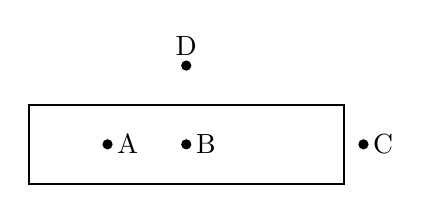
\begin{tikzpicture}
          \draw[thick] rectangle (4,1);
          \fill (1,.5) circle (.065) node[right]{A};
          \fill (2,.5) circle (.065) node[right]{B};
          \fill (4.25,.5) circle (.065) node[right]{C};
          \fill (2,1.5) circle (.065) node[above]{D};
        \end{tikzpicture}
      \end{center}
      \vspace{.15in}
    }

    \part From the choices below, \textbf{select} the point where you would
    place a magnetic field probe (a probe that can measure the magnitude of the
    magnetic field) to best measure the strength of the magnetic field of the
    solenoid in order to determine the vacuum permeability $\mu_0$.

    \vspace{.1in}
    \underline{\hspace{.3in}} A\hspace{.5in}
    \underline{\hspace{.3in}} B\hspace{.5in}
    \underline{\hspace{.3in}} C\hspace{.5in}
    \underline{\hspace{.3in}} D

    \vspace{.15in}\textbf{Justify} your answer based on the model for a simple
    solenoid.
    \newpage
    
    \uplevel{
      The figures below show two different solenoids that will be connected in
      the circuit above. Solenoid 1 has a length $\ell=\SI{25}{\centi\metre}$
      with $N=100$ turns. Solenoid 2 has a length $\ell=\SI{5.}{\centi\metre}$
      with $N=5$ turns.
      \begin{center}
        \pic{.5}{2solenoids}
        
        \underline{Note:} Figures not drawn to scale.
      \end{center}
      
      \vspace{.1in}A graph of the magnitude of the magnetic field $B$ as a
      function of $NI/\ell$ is shown below. The best-fit lines for the data are
      shown as a solid line for solenoid 1 and as a dashed line for solenoid 2.
      
      \cpic{.85}{results}
    }

    \part Which solenoid's best-fit line would give the best results for
    determining a value for the vacuum permeability $\mu_0$?
 
    \vspace{.1in}
    \underline{\hspace{.3in}} Solenoid 1\hspace{.5in}
    \underline{\hspace{.3in}} Solenoid 2

    \vspace{.15in}\textbf{Justify} your answer.
    \newpage
    
    \part Use the slope of the best-fit line for the solenoid chosen in part
    \textbf{D} to \textbf{estimate} value of the vacuum permeability $\mu_o$.
    \vspace{\stretch1}
    
    \part\textbf{Calculate} the percent error for the experimental value of the
    vacuum permeability $\mu_0$ determined in part \textbf{E}.
    \vspace{\stretch1}
    
    \part What is a reasonable physical explanation for a best-fit line that
    does not pass through the origin?
    \vspace{\stretch1}
    
    \part Suppose a student connects the solenoid in a closed circuit similar
    to the circuit in part \textbf{A} but without the resistor. The student
    notices the multimeter stops functioning after the power supply is turned
    on. \textbf{Explain} what causes the failure of the multimeter.
    \vspace{\stretch1}
  \end{parts}



\end{questions}
\end{document}
